\documentclass[DM,authoryear,toc]{lsstdoc}
\input{meta}

% Package imports go here.

% Local commands go here.

%If you want glossaries
%\input{aglossary.tex}
%\makeglossaries

\title{Report on the performance of image differencing from the perspective of the learning-based classifier task}

% Optional subtitle
% \setDocSubtitle{A subtitle}

\author{%
Nima Sedaghat
}

\setDocRef{DMTN-274}
\setDocUpstreamLocation{\url{https://github.com/lsst-dm/dmtn-274}}

\date{\vcsDate}

% Optional: name of the document's curator
% \setDocCurator{The Curator of this Document}

\setDocAbstract{%
The output of the image differencing task (subtractImages combined with detectAndMeasure) is the input to the learning based classification module (rbClassifier) in AP pipelines. Therefore, the quality of the generated difference images and the detected sources, is of a high importance from the classifier's point of view. This tech-note tries to provide a basic statistical analysis of this data product as generated with the current version of the AP pipeline. Obviously, the classifier itself is not involved neither in the pipelines nor the analysis provided in this report.
}

% Change history defined here.
% Order: oldest first.
% Fields: VERSION, DATE, DESCRIPTION, OWNER NAME.
% See LPM-51 for version number policy.
\setDocChangeRecord{%
  \addtohist{1}{YYYY-MM-DD}{Unreleased.}{Nima Sedaghat}
}


\begin{document}

% Create the title page.
\maketitle
% Frequently for a technote we do not want a title page  uncomment this to remove the title page and changelog.
% use \mkshorttitle to remove the extra pages

% ADD CONTENT HERE
% You can also use the \input command to include several content files.

\section{Experiment Setup}
\subsection{Pipeline}
In this experiment we simply pass raw images through the AP pipeline (\emph{without} running the rbClassification task) to get difference images and the corresponding sources.

\begin{figure}[h]
  \centering
  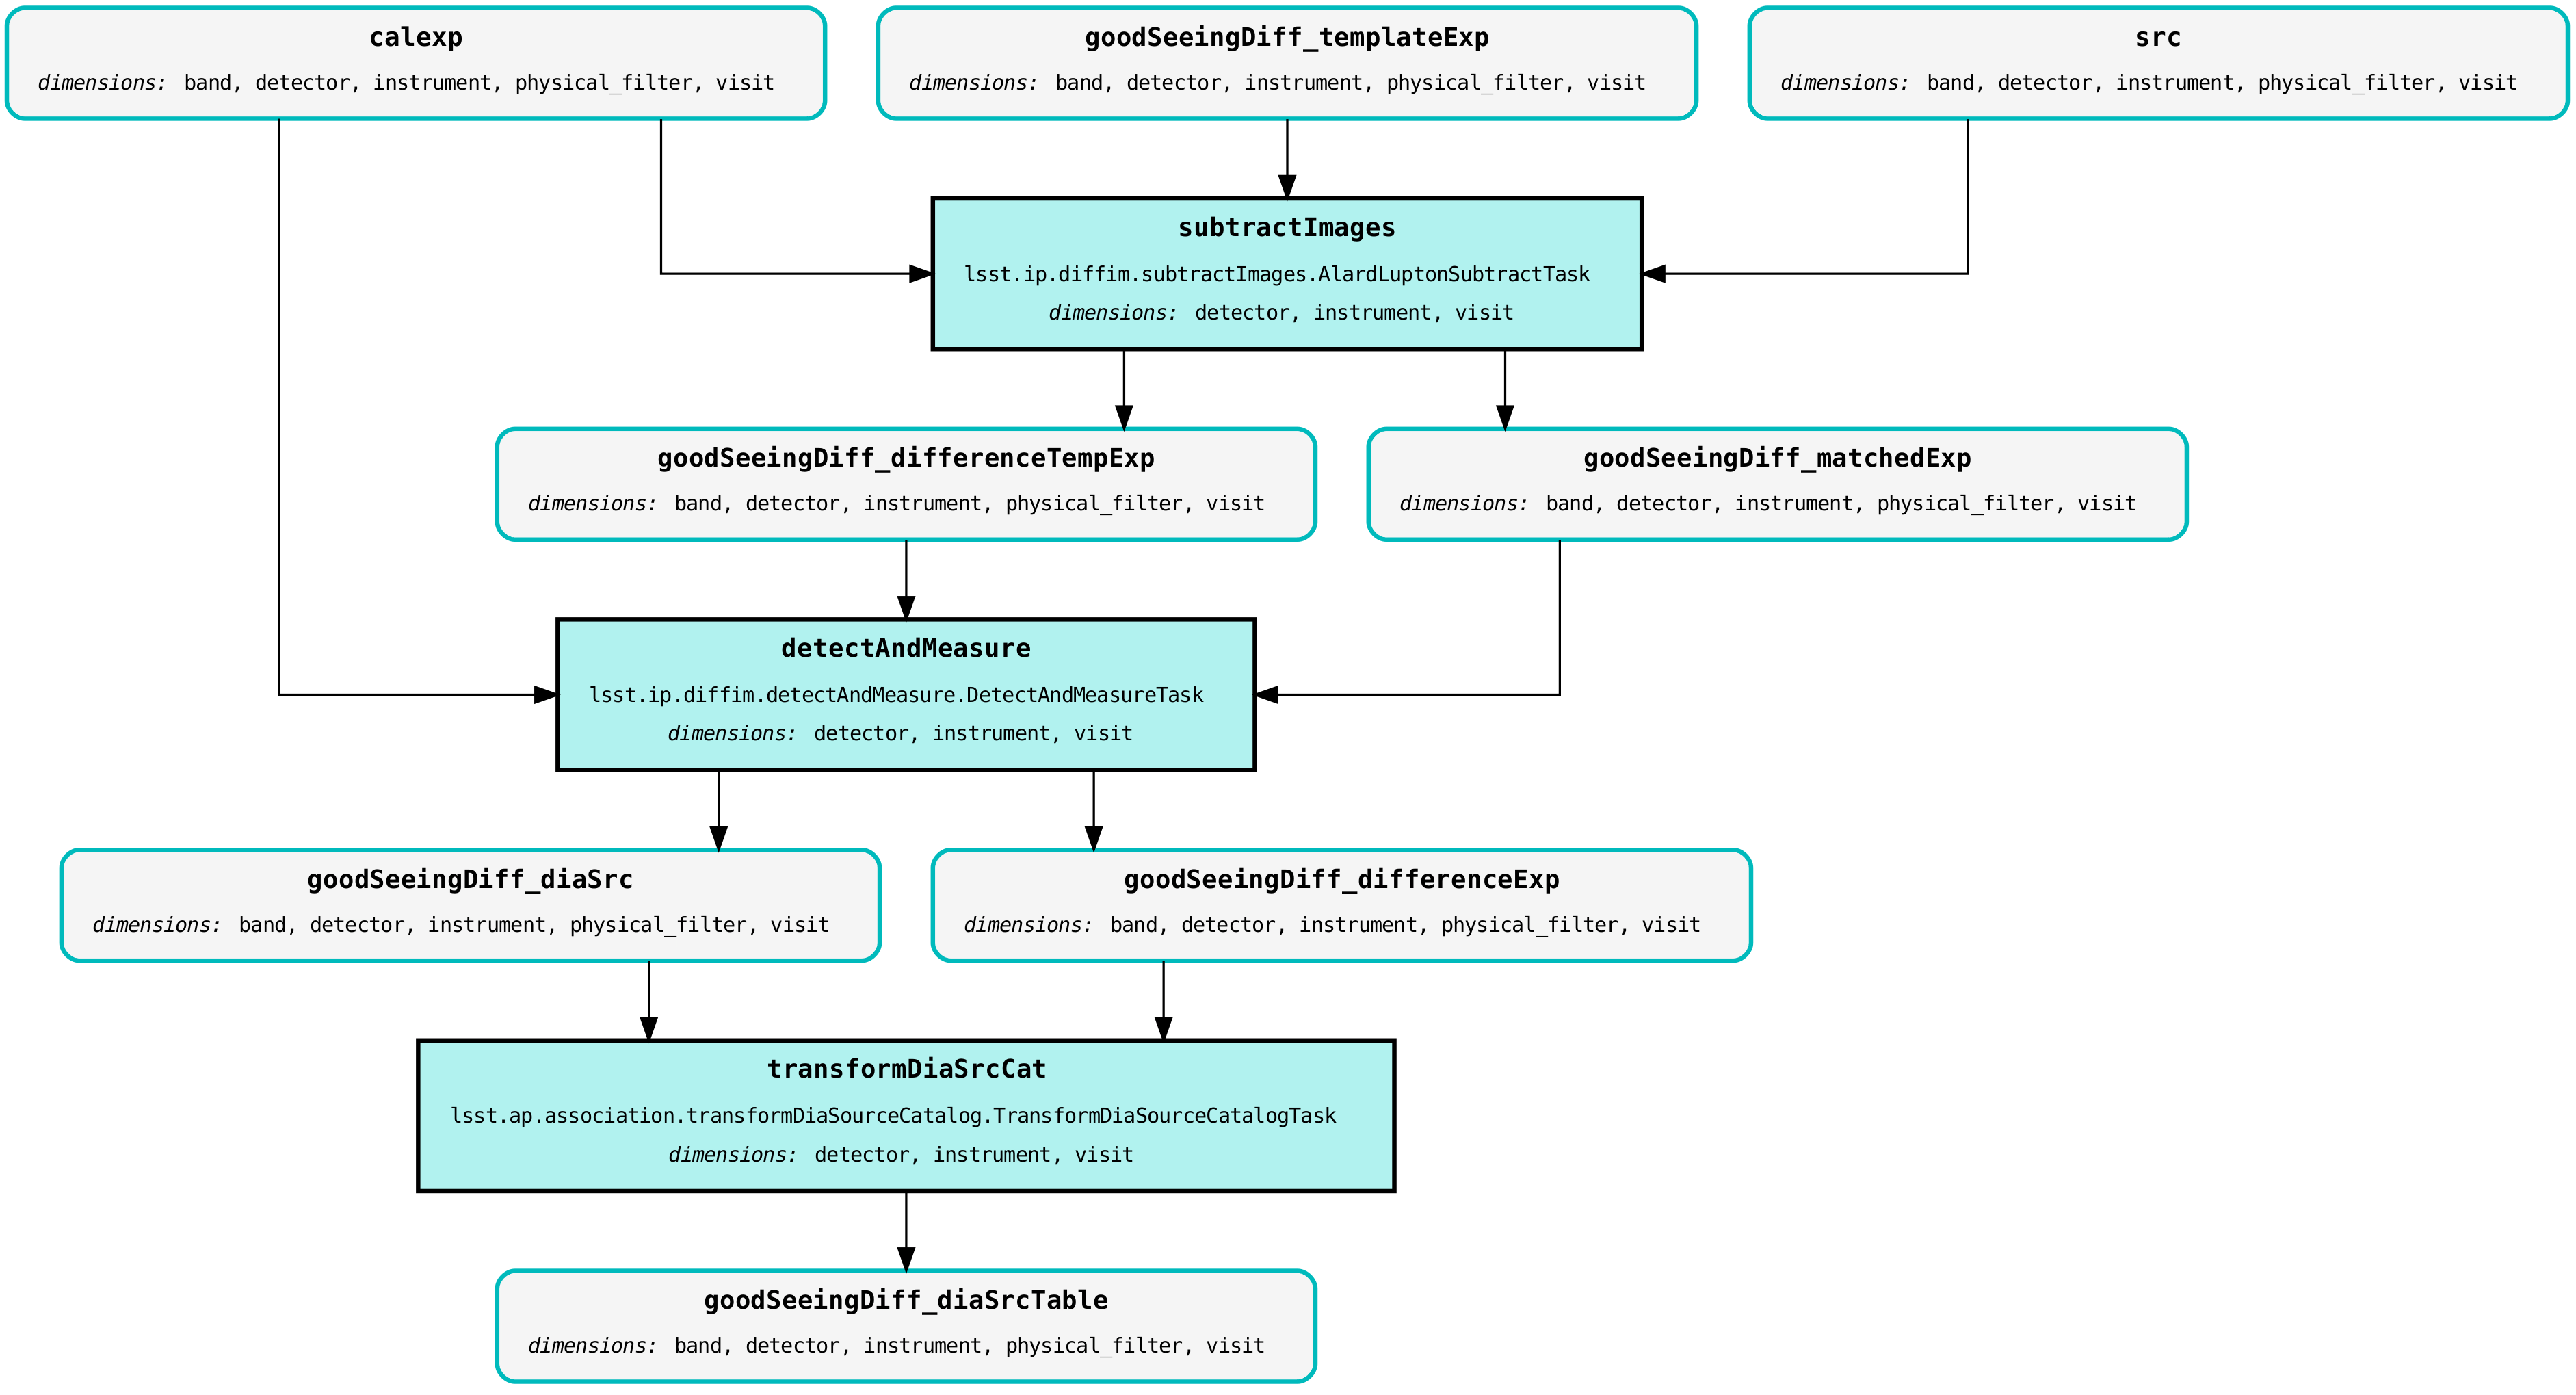
\includegraphics[width=0.9\textwidth]{pipeline.png}
  \caption{The lower part of the pipeline used for assessing the performance of the image differencing task. Note that the ``rbClassifier'' has been removed from the pipeline.}
  \label{fig:exposure_hist}
\end{figure}

The \texttt{transformDiaSrcCat} is kept in the pipeline, so the ``sky\_source'' are removed and do not clutter our data.
We used the \texttt{w\_2023\_38} version of the stack throughout the experiment.

\subsection{Data}
We use data from DC2, so that we have access to the corresponding truth labels. We use exposures from tract \texttt{3080} through the pipeline, and use \texttt{dataIds} of the first 50 of them, as returned by the \texttt{butler} query, to fetch the sample set of detected sources and relevant ground truth for this experiment -- the list is pasted in appendix~\ref{app:ids}

\subsection{Evaluation Results}
\begin{verbatim}
Number of diaSources:  4373
Number of sources matching the truth:  346
Number of sources NOT matching the truth (false positives):  4027

Total number of truth objects:  5258
Number of truth objects not matched to a source (misses):  4912
\end{verbatim}

According to the about numbers, \underline{$93.4\%$ of the real transients are ``missed forever''}: they haven't survived the upstream task and so do not make it to the real-bogus classifier at all.
Figure~\ref{fig:distributions} illustrates the distributions of \texttt{mag\_r} and \texttt{delta\_flux} for these real (true) transients.

\begin{figure}[h]
  \centering
  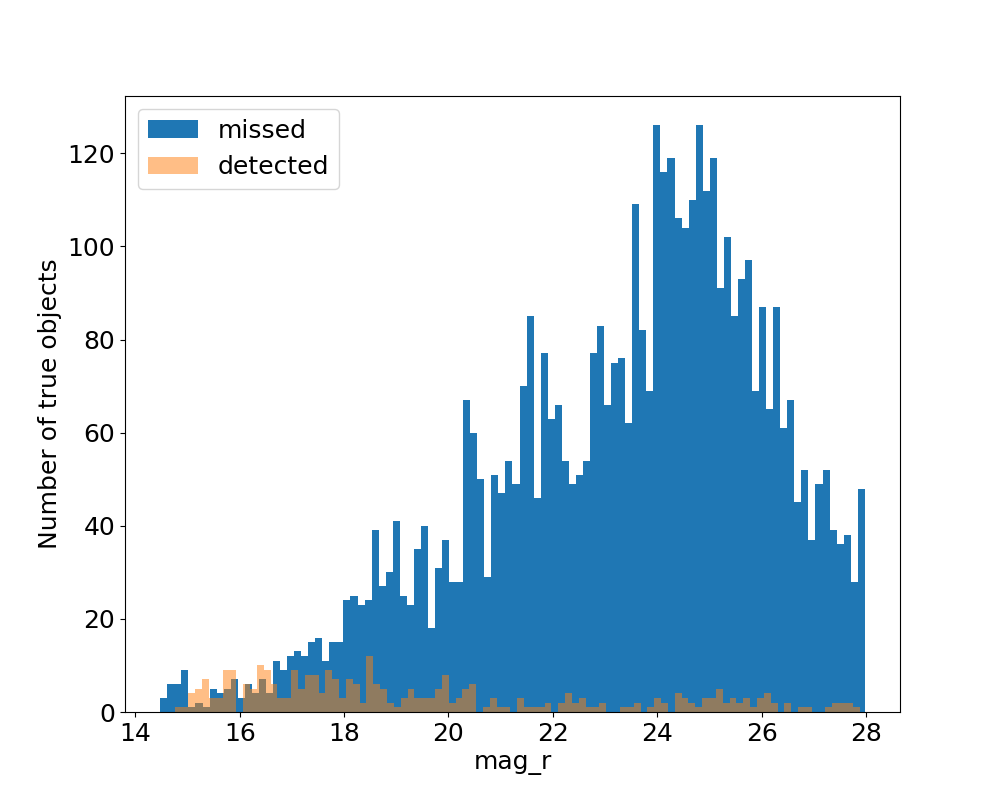
\includegraphics[width=0.4\textwidth]{mag_r_hist.png}
  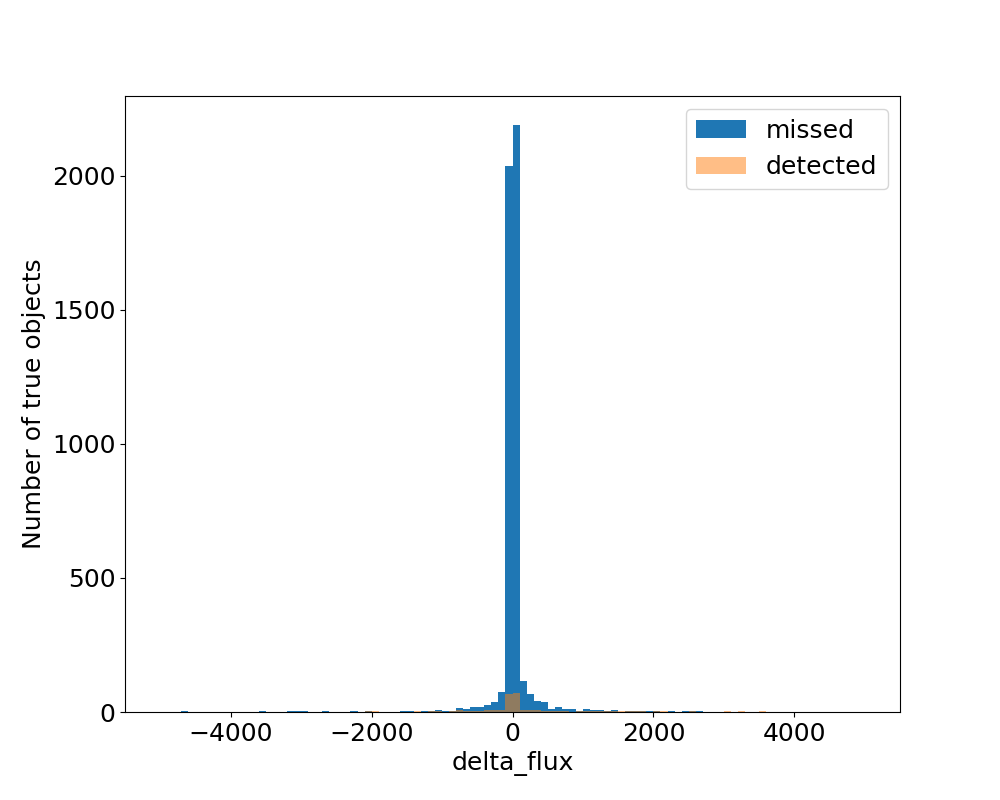
\includegraphics[width=0.4\textwidth]{delta_flux_hist.png}
  \caption{Distributions of \texttt{mag\_r} and \texttt{delta\_flux} of true transient objects.}
  \label{fig:distributions}
\end{figure}

\clearpage

\begin{figure}[h]
  \centering
  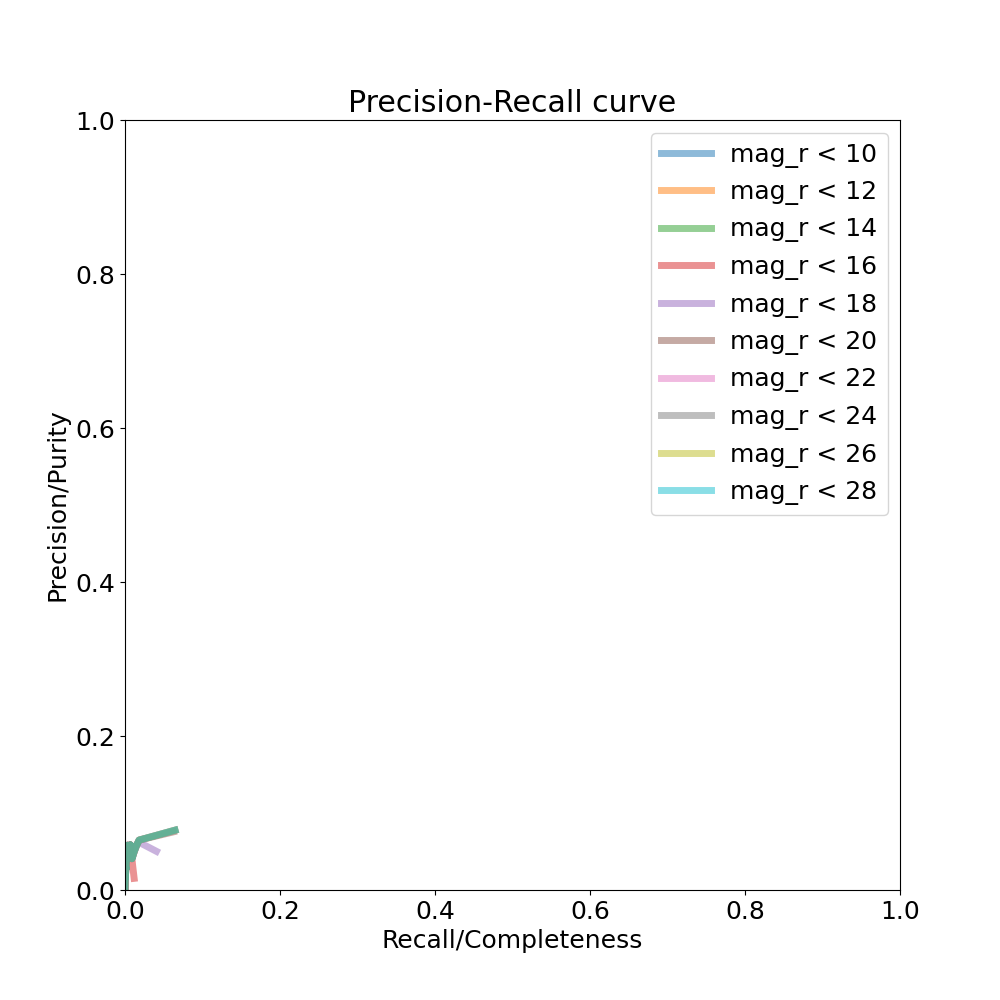
\includegraphics[width=0.4\textwidth]{precision_recall_curve}
  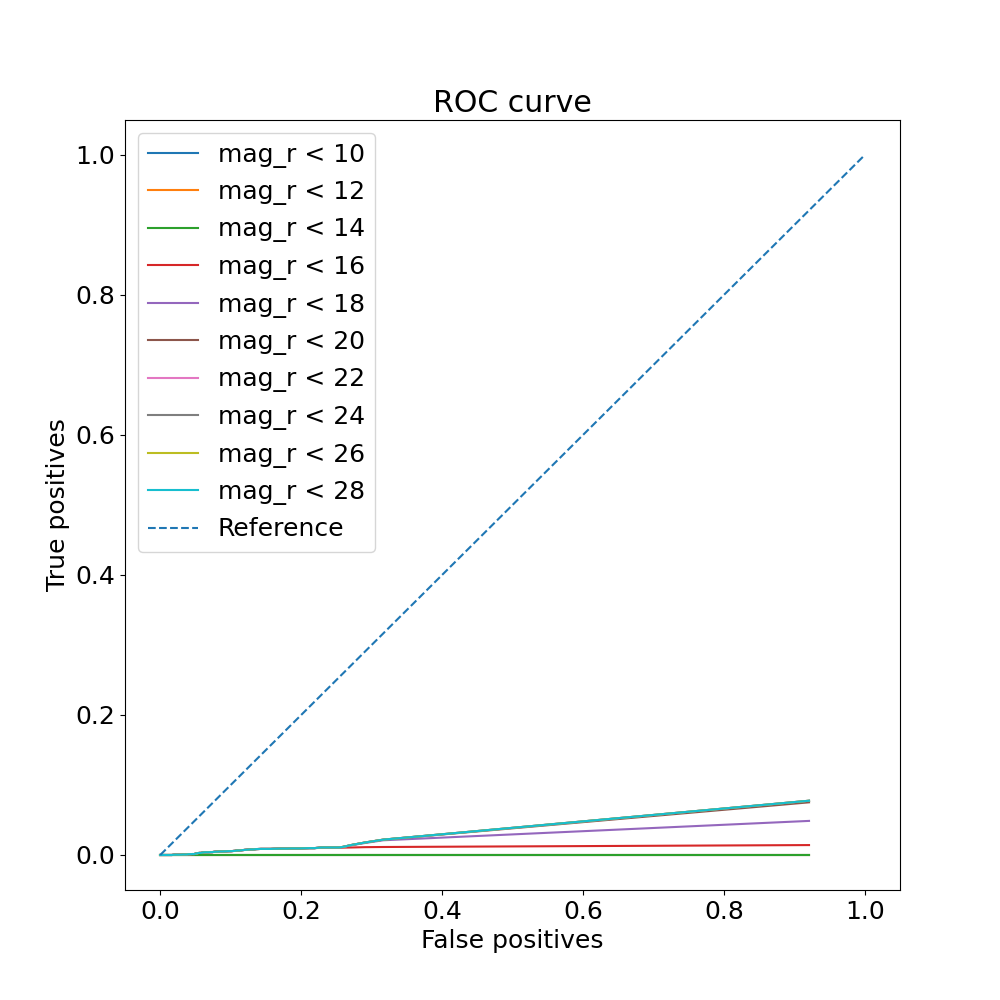
\includegraphics[width=0.4\textwidth]{roc_curve}
  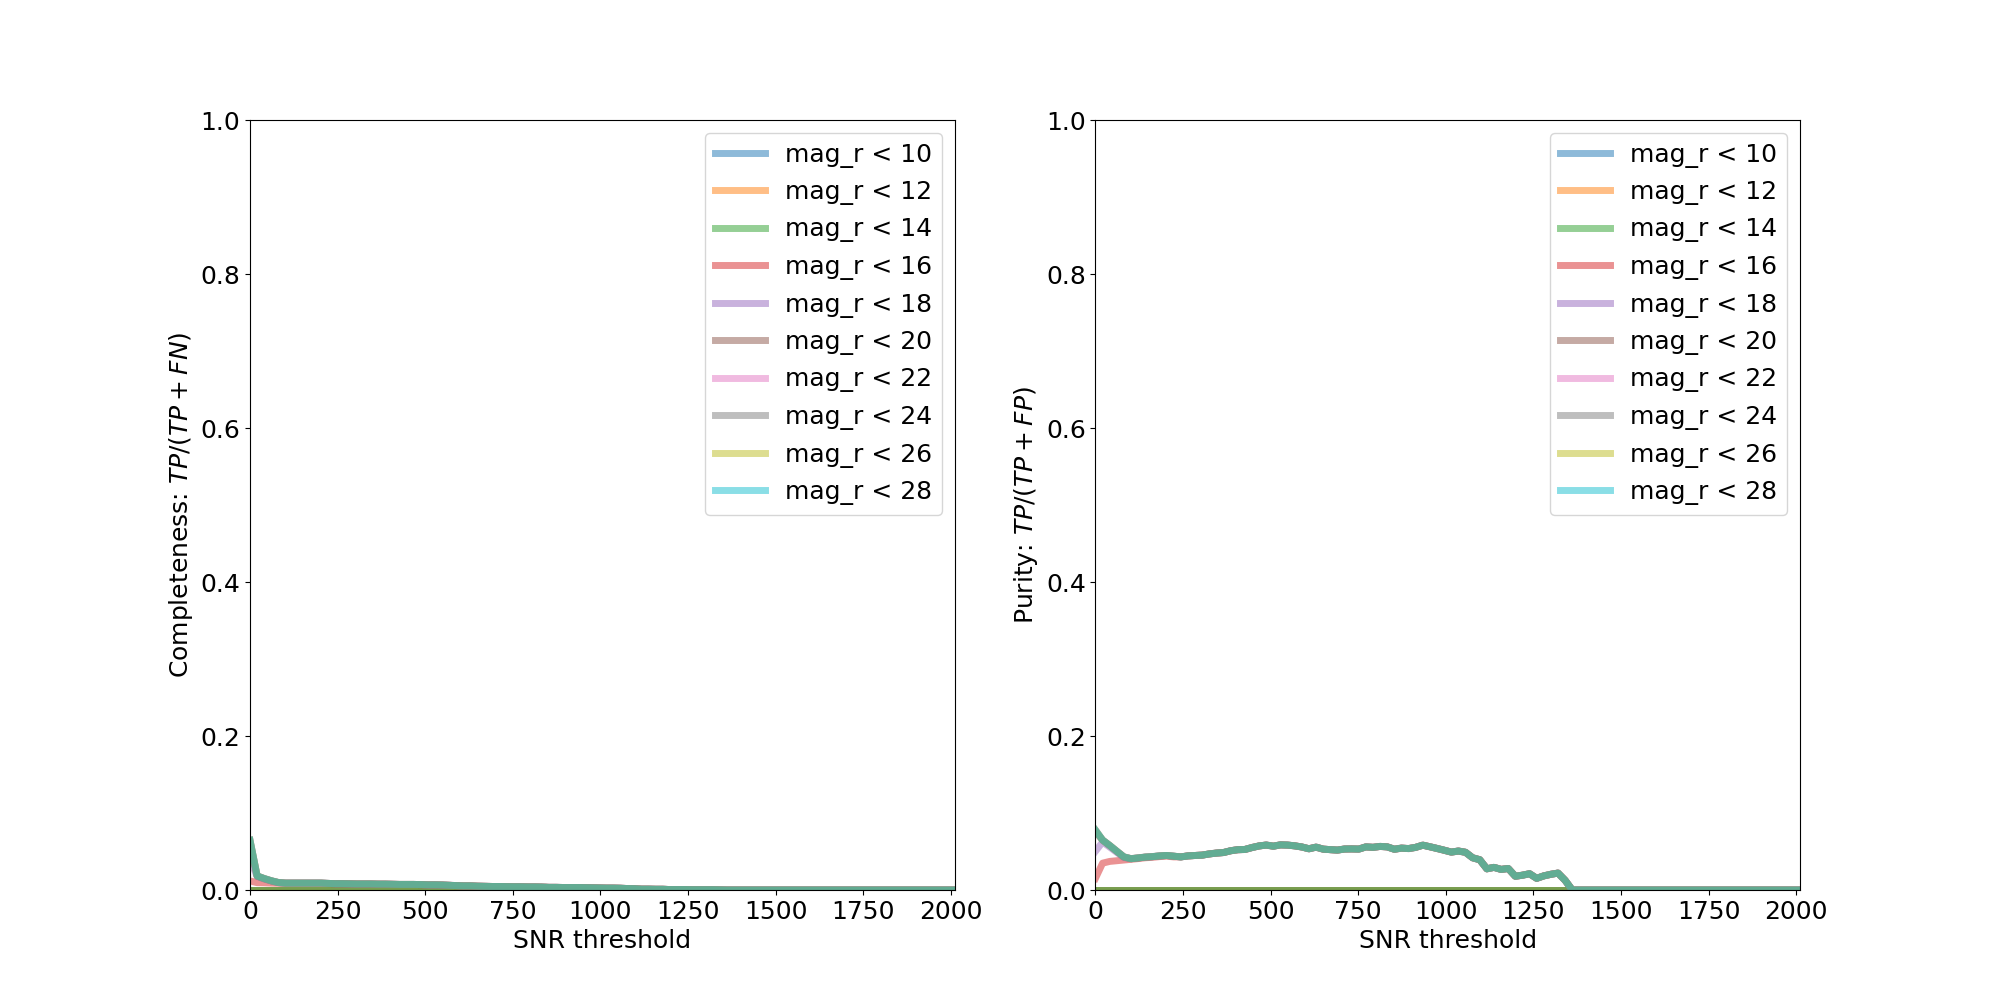
\includegraphics[width=0.9\textwidth]{detection_rate}
  \caption{Various evaluation curves providing different viewpoints on the performance of the model. Each plot is generated using various higher bounds on the magnitude, to assess the effect of faint/brightness on the results.}
  \label{fig:evals}
\end{figure}

The unfamiliar behavior of the evaluation plots in Figure~\ref{fig:evals} is due, in part, to the the extremely high percentage of missed objects resulting from the threshold applied to the output of the difference image, not allowing for the curves to meet the $100\%$ recall level at any point. A similar observation has been reported in August 2022 -- see Figure~\ref{fig:slack}

\clearpage
\begin{figure}[h]
  \centering
  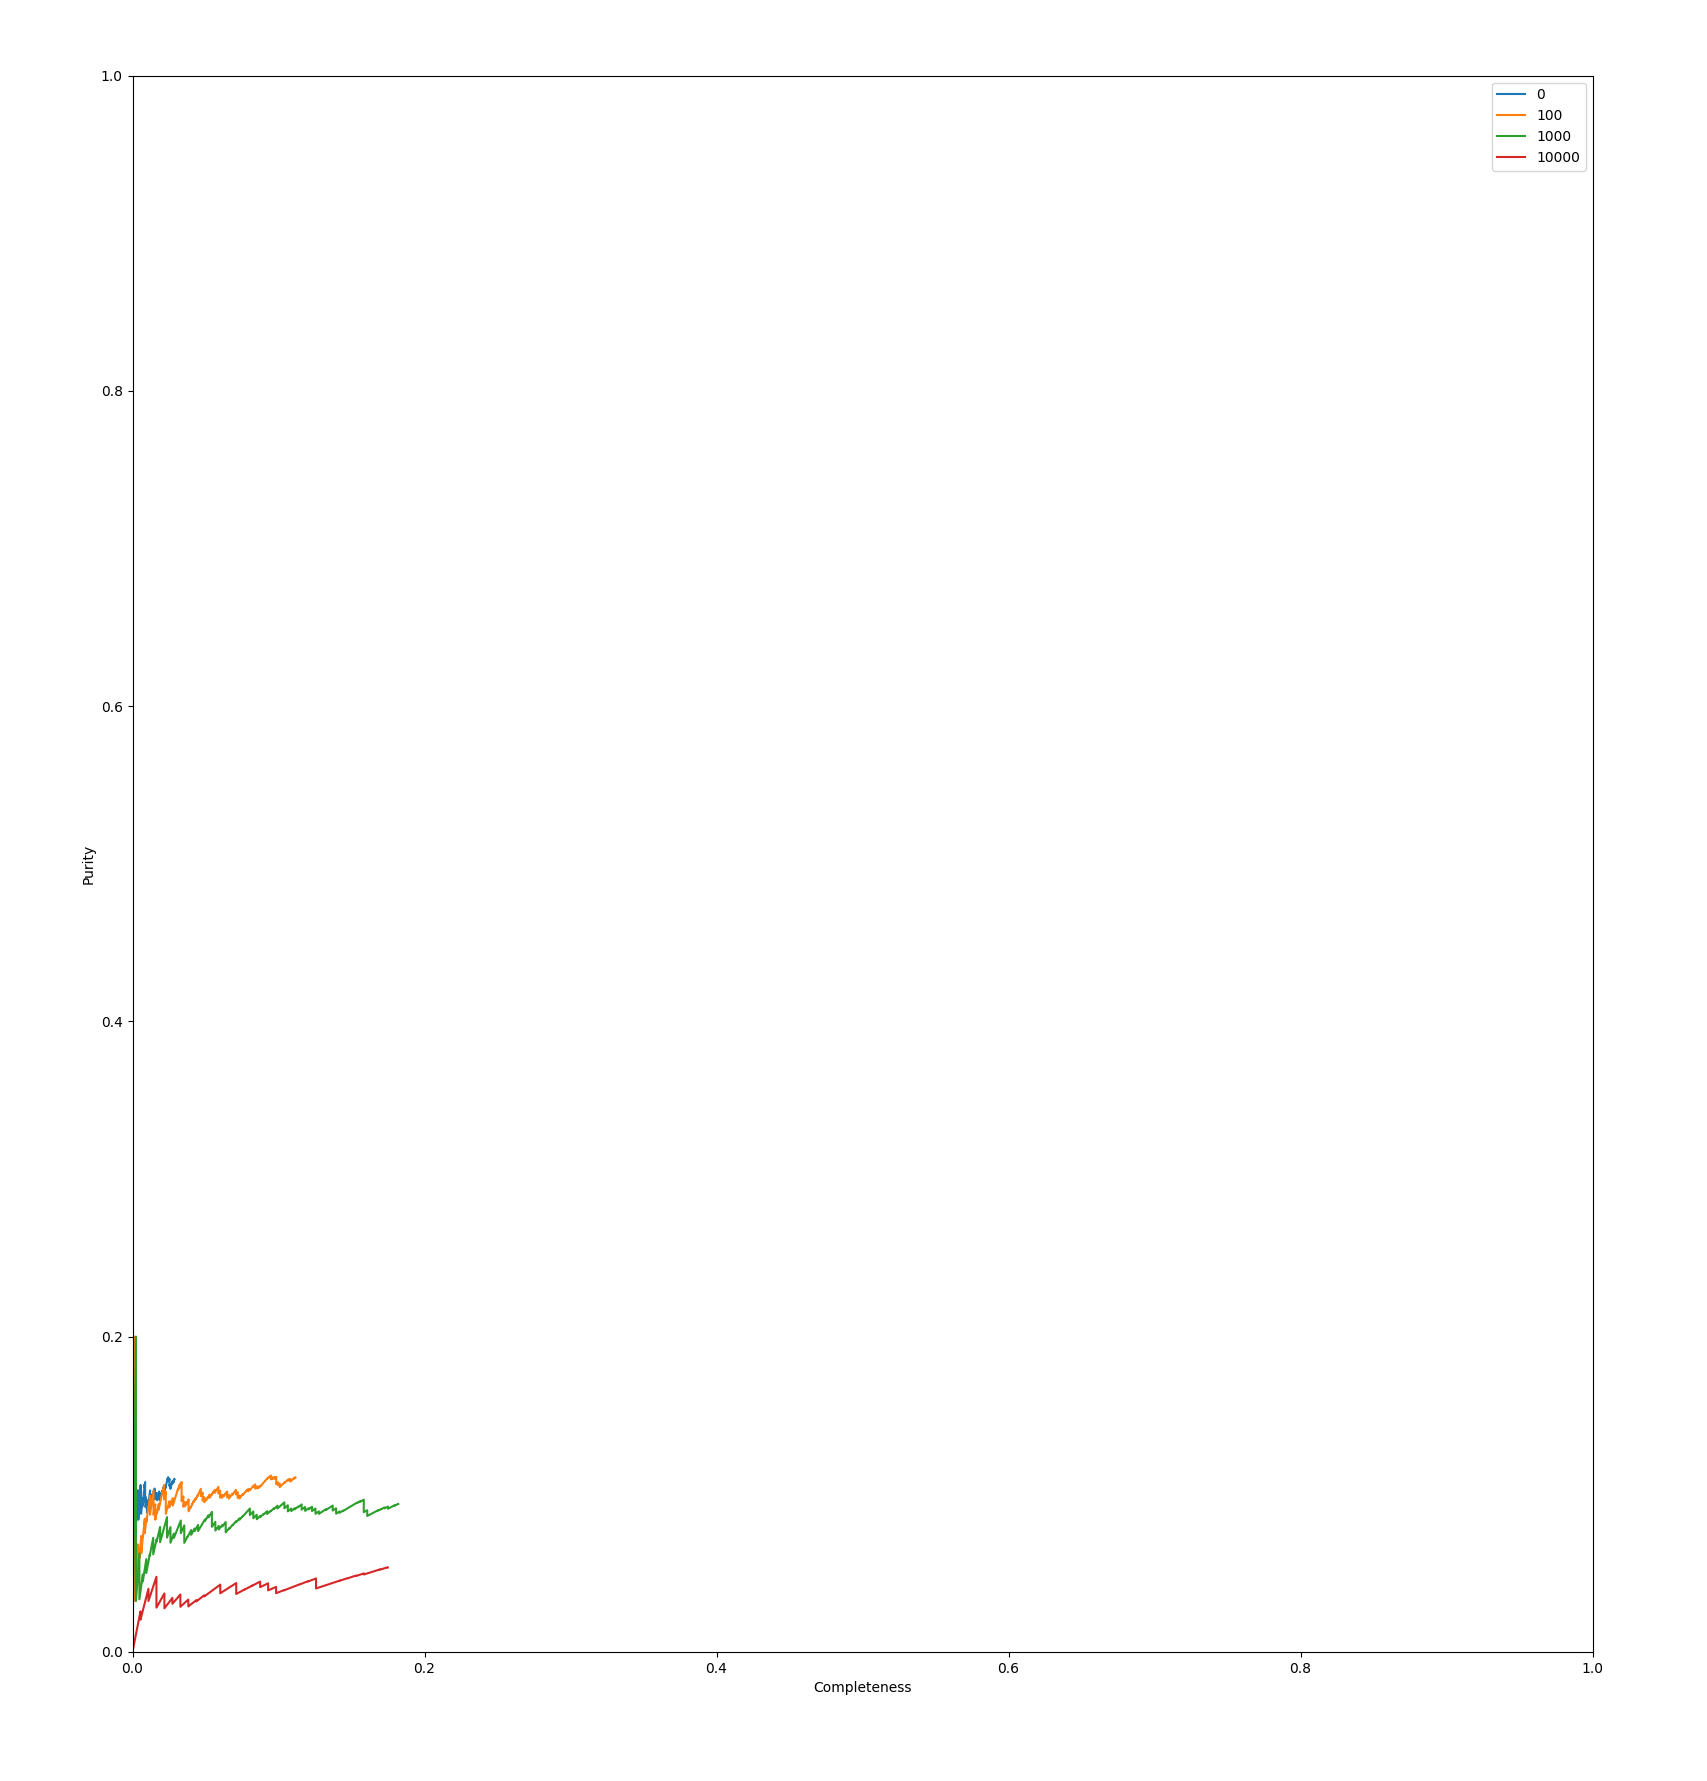
\includegraphics[width=0.4\textwidth]{slack}
  \caption{The similar evaluation curves that have been observed back in August 2022 -- Please see \url{https://lsstc.slack.com/archives/C2B6X08LS/p1659393708935119}. Different colors correpond to different \texttt{delta\_flux} values. The fonts sizes are indeed too small for a printed document, but the idea is to keep the original image intact.}
  \label{fig:slack}
\end{figure}

The fact that any such loss is inevitably passed down to the downstream real-bogus classifier has also been theoretically predicted in section 3.2 of DMTN-216. Note that decreasing the threshold applied to the difference image is not a solution for the issue described above. Lowering the threshold would indeed lead to a drastic increase in false positives, and even if a higher recall may be seen in the curves, it will be only at precisions close to zero: the main intention behind the use of thresholding in the current pipeline.

\clearpage

\appendix
\section{List of dataIds}
\label{app:ids}
\begin{lstlisting}[language=Python, basicstyle=\tiny]
dataId={'band': 'i', 'instrument': 'LSSTCam-imSim', 'detector': 151, 'physical_filter': 'i_sim_1.4', 'visit': 1030665} records=None
dataId={'band': 'g', 'instrument': 'LSSTCam-imSim', 'detector': 45, 'physical_filter': 'g_sim_1.4', 'visit': 1039948} records=None
dataId={'band': 'y', 'instrument': 'LSSTCam-imSim', 'detector': 21, 'physical_filter': 'y_sim_1.4', 'visit': 1010524} records=None
dataId={'band': 'y', 'instrument': 'LSSTCam-imSim', 'detector': 156, 'physical_filter': 'y_sim_1.4', 'visit': 1012086} records=None
dataId={'band': 'i', 'instrument': 'LSSTCam-imSim', 'detector': 72, 'physical_filter': 'i_sim_1.4', 'visit': 1030670} records=None
dataId={'band': 'r', 'instrument': 'LSSTCam-imSim', 'detector': 171, 'physical_filter': 'r_sim_1.4', 'visit': 1006059} records=None
dataId={'band': 'y', 'instrument': 'LSSTCam-imSim', 'detector': 30, 'physical_filter': 'y_sim_1.4', 'visit': 647595} records=None
dataId={'band': 'i', 'instrument': 'LSSTCam-imSim', 'detector': 114, 'physical_filter': 'i_sim_1.4', 'visit': 1013711} records=None
dataId={'band': 'g', 'instrument': 'LSSTCam-imSim', 'detector': 66, 'physical_filter': 'g_sim_1.4', 'visit': 1019980} records=None
dataId={'band': 'r', 'instrument': 'LSSTCam-imSim', 'detector': 18, 'physical_filter': 'r_sim_1.4', 'visit': 1052891} records=None
dataId={'band': 'i', 'instrument': 'LSSTCam-imSim', 'detector': 92, 'physical_filter': 'i_sim_1.4', 'visit': 1030665} records=None
dataId={'band': 'r', 'instrument': 'LSSTCam-imSim', 'detector': 44, 'physical_filter': 'r_sim_1.4', 'visit': 1052890} records=None
dataId={'band': 'i', 'instrument': 'LSSTCam-imSim', 'detector': 45, 'physical_filter': 'i_sim_1.4', 'visit': 1013734} records=None
dataId={'band': 'r', 'instrument': 'LSSTCam-imSim', 'detector': 138, 'physical_filter': 'r_sim_1.4', 'visit': 1052890} records=None
dataId={'band': 'y', 'instrument': 'LSSTCam-imSim', 'detector': 28, 'physical_filter': 'y_sim_1.4', 'visit': 1032264} records=None
dataId={'band': 'y', 'instrument': 'LSSTCam-imSim', 'detector': 5, 'physical_filter': 'y_sim_1.4', 'visit': 1032264} records=None
dataId={'band': 'y', 'instrument': 'LSSTCam-imSim', 'detector': 115, 'physical_filter': 'y_sim_1.4', 'visit': 646755} records=None
dataId={'band': 'r', 'instrument': 'LSSTCam-imSim', 'detector': 147, 'physical_filter': 'r_sim_1.4', 'visit': 1049332} records=None
dataId={'band': 'i', 'instrument': 'LSSTCam-imSim', 'detector': 29, 'physical_filter': 'i_sim_1.4', 'visit': 1029810} records=None
dataId={'band': 'r', 'instrument': 'LSSTCam-imSim', 'detector': 165, 'physical_filter': 'r_sim_1.4', 'visit': 638950} records=None
dataId={'band': 'i', 'instrument': 'LSSTCam-imSim', 'detector': 164, 'physical_filter': 'i_sim_1.4', 'visit': 1030665} records=None
dataId={'band': 'y', 'instrument': 'LSSTCam-imSim', 'detector': 8, 'physical_filter': 'y_sim_1.4', 'visit': 1032264} records=None
dataId={'band': 'i', 'instrument': 'LSSTCam-imSim', 'detector': 121, 'physical_filter': 'i_sim_1.4', 'visit': 645623} records=None
dataId={'band': 'r', 'instrument': 'LSSTCam-imSim', 'detector': 141, 'physical_filter': 'r_sim_1.4', 'visit': 1052890} records=None
dataId={'band': 'r', 'instrument': 'LSSTCam-imSim', 'detector': 93, 'physical_filter': 'r_sim_1.4', 'visit': 1052890} records=None
dataId={'band': 'i', 'instrument': 'LSSTCam-imSim', 'detector': 24, 'physical_filter': 'i_sim_1.4', 'visit': 1030664} records=None
dataId={'band': 'y', 'instrument': 'LSSTCam-imSim', 'detector': 59, 'physical_filter': 'y_sim_1.4', 'visit': 1033987} records=None
dataId={'band': 'r', 'instrument': 'LSSTCam-imSim', 'detector': 14, 'physical_filter': 'r_sim_1.4', 'visit': 1006099} records=None
dataId={'band': 'i', 'instrument': 'LSSTCam-imSim', 'detector': 184, 'physical_filter': 'i_sim_1.4', 'visit': 1030666} records=None
dataId={'band': 'y', 'instrument': 'LSSTCam-imSim', 'detector': 164, 'physical_filter': 'y_sim_1.4', 'visit': 1056411} records=None
dataId={'band': 'r', 'instrument': 'LSSTCam-imSim', 'detector': 83, 'physical_filter': 'r_sim_1.4', 'visit': 1052890} records=None
dataId={'band': 'i', 'instrument': 'LSSTCam-imSim', 'detector': 11, 'physical_filter': 'i_sim_1.4', 'visit': 1029805} records=None
dataId={'band': 'r', 'instrument': 'LSSTCam-imSim', 'detector': 38, 'physical_filter': 'r_sim_1.4', 'visit': 1052890} records=None
dataId={'band': 'g', 'instrument': 'LSSTCam-imSim', 'detector': 62, 'physical_filter': 'g_sim_1.4', 'visit': 1039916} records=None
dataId={'band': 'r', 'instrument': 'LSSTCam-imSim', 'detector': 167, 'physical_filter': 'r_sim_1.4', 'visit': 1038217} records=None
dataId={'band': 'y', 'instrument': 'LSSTCam-imSim', 'detector': 180, 'physical_filter': 'y_sim_1.4', 'visit': 1033109} records=None
dataId={'band': 'r', 'instrument': 'LSSTCam-imSim', 'detector': 184, 'physical_filter': 'r_sim_1.4', 'visit': 1006059} records=None
dataId={'band': 'r', 'instrument': 'LSSTCam-imSim', 'detector': 129, 'physical_filter': 'r_sim_1.4', 'visit': 1006007} records=None
dataId={'band': 'i', 'instrument': 'LSSTCam-imSim', 'detector': 17, 'physical_filter': 'i_sim_1.4', 'visit': 1030664} records=None
dataId={'band': 'y', 'instrument': 'LSSTCam-imSim', 'detector': 80, 'physical_filter': 'y_sim_1.4', 'visit': 1032264} records=None
dataId={'band': 'r', 'instrument': 'LSSTCam-imSim', 'detector': 3, 'physical_filter': 'r_sim_1.4', 'visit': 1027069} records=None
dataId={'band': 'i', 'instrument': 'LSSTCam-imSim', 'detector': 92, 'physical_filter': 'i_sim_1.4', 'visit': 645659} records=None
dataId={'band': 'g', 'instrument': 'LSSTCam-imSim', 'detector': 111, 'physical_filter': 'g_sim_1.4', 'visit': 1039916} records=None
dataId={'band': 'i', 'instrument': 'LSSTCam-imSim', 'detector': 70, 'physical_filter': 'i_sim_1.4', 'visit': 1029805} records=None
dataId={'band': 'y', 'instrument': 'LSSTCam-imSim', 'detector': 113, 'physical_filter': 'y_sim_1.4', 'visit': 1032265} records=None
dataId={'band': 'y', 'instrument': 'LSSTCam-imSim', 'detector': 154, 'physical_filter': 'y_sim_1.4', 'visit': 646755} records=None
dataId={'band': 'r', 'instrument': 'LSSTCam-imSim', 'detector': 69, 'physical_filter': 'r_sim_1.4', 'visit': 1006099} records=None
dataId={'band': 'r', 'instrument': 'LSSTCam-imSim', 'detector': 170, 'physical_filter': 'r_sim_1.4', 'visit': 1038217} records=None
dataId={'band': 'r', 'instrument': 'LSSTCam-imSim', 'detector': 18, 'physical_filter': 'r_sim_1.4', 'visit': 1049334} records=None
dataId={'band': 'i', 'instrument': 'LSSTCam-imSim', 'detector': 132, 'physical_filter': 'i_sim_1.4', 'visit': 645659} records=None
dataId={'band': 'i', 'instrument': 'LSSTCam-imSim', 'detector': 180, 'physical_filter': 'i_sim_1.4', 'visit': 1030665} records=None
dataId={'band': 'y', 'instrument': 'LSSTCam-imSim', 'detector': 31, 'physical_filter': 'y_sim_1.4', 'visit': 1032264} records=None
dataId={'band': 'y', 'instrument': 'LSSTCam-imSim', 'detector': 101, 'physical_filter': 'y_sim_1.4', 'visit': 1012178} records=None
dataId={'band': 'r', 'instrument': 'LSSTCam-imSim', 'detector': 148, 'physical_filter': 'r_sim_1.4', 'visit': 1049335} records=None
dataId={'band': 'i', 'instrument': 'LSSTCam-imSim', 'detector': 10, 'physical_filter': 'i_sim_1.4', 'visit': 1013734} records=None
dataId={'band': 'r', 'instrument': 'LSSTCam-imSim', 'detector': 55, 'physical_filter': 'r_sim_1.4', 'visit': 1038222} records=None
dataId={'band': 'y', 'instrument': 'LSSTCam-imSim', 'detector': 93, 'physical_filter': 'y_sim_1.4', 'visit': 1032264} records=None
dataId={'band': 'g', 'instrument': 'LSSTCam-imSim', 'detector': 101, 'physical_filter': 'g_sim_1.4', 'visit': 1039916} records=None
dataId={'band': 'y', 'instrument': 'LSSTCam-imSim', 'detector': 137, 'physical_filter': 'y_sim_1.4', 'visit': 1012086} records=None
dataId={'band': 'i', 'instrument': 'LSSTCam-imSim', 'detector': 30, 'physical_filter': 'i_sim_1.4', 'visit': 1029810} records=None
dataId={'band': 'i', 'instrument': 'LSSTCam-imSim', 'detector': 100, 'physical_filter': 'i_sim_1.4', 'visit': 1013734} records=None
dataId={'band': 'i', 'instrument': 'LSSTCam-imSim', 'detector': 21, 'physical_filter': 'i_sim_1.4', 'visit': 1030664} records=None
dataId={'band': 'i', 'instrument': 'LSSTCam-imSim', 'detector': 77, 'physical_filter': 'i_sim_1.4', 'visit': 645659} records=None
dataId={'band': 'i', 'instrument': 'LSSTCam-imSim', 'detector': 115, 'physical_filter': 'i_sim_1.4', 'visit': 1029804} records=None
dataId={'band': 'i', 'instrument': 'LSSTCam-imSim', 'detector': 163, 'physical_filter': 'i_sim_1.4', 'visit': 1030669} records=None
dataId={'band': 'r', 'instrument': 'LSSTCam-imSim', 'detector': 41, 'physical_filter': 'r_sim_1.4', 'visit': 1052890} records=None
dataId={'band': 'i', 'instrument': 'LSSTCam-imSim', 'detector': 129, 'physical_filter': 'i_sim_1.4', 'visit': 645659} records=None
dataId={'band': 'r', 'instrument': 'LSSTCam-imSim', 'detector': 145, 'physical_filter': 'r_sim_1.4', 'visit': 1049335} records=None
dataId={'band': 'y', 'instrument': 'LSSTCam-imSim', 'detector': 174, 'physical_filter': 'y_sim_1.4', 'visit': 1056411} records=None
dataId={'band': 'y', 'instrument': 'LSSTCam-imSim', 'detector': 115, 'physical_filter': 'y_sim_1.4', 'visit': 1012086} records=None
dataId={'band': 'i', 'instrument': 'LSSTCam-imSim', 'detector': 36, 'physical_filter': 'i_sim_1.4', 'visit': 1029810} records=None
dataId={'band': 'g', 'instrument': 'LSSTCam-imSim', 'detector': 24, 'physical_filter': 'g_sim_1.4', 'visit': 1039916} records=None
dataId={'band': 'r', 'instrument': 'LSSTCam-imSim', 'detector': 66, 'physical_filter': 'r_sim_1.4', 'visit': 1006099} records=None
dataId={'band': 'r', 'instrument': 'LSSTCam-imSim', 'detector': 94, 'physical_filter': 'r_sim_1.4', 'visit': 1038222} records=None
dataId={'band': 'g', 'instrument': 'LSSTCam-imSim', 'detector': 82, 'physical_filter': 'g_sim_1.4', 'visit': 1039948} records=None
dataId={'band': 'i', 'instrument': 'LSSTCam-imSim', 'detector': 129, 'physical_filter': 'i_sim_1.4', 'visit': 1030665} records=None
dataId={'band': 'y', 'instrument': 'LSSTCam-imSim', 'detector': 153, 'physical_filter': 'y_sim_1.4', 'visit': 1033987} records=None
dataId={'band': 'r', 'instrument': 'LSSTCam-imSim', 'detector': 39, 'physical_filter': 'r_sim_1.4', 'visit': 1006037} records=None
dataId={'band': 'i', 'instrument': 'LSSTCam-imSim', 'detector': 26, 'physical_filter': 'i_sim_1.4', 'visit': 1029776} records=None
dataId={'band': 'r', 'instrument': 'LSSTCam-imSim', 'detector': 25, 'physical_filter': 'r_sim_1.4', 'visit': 1049334} records=None
dataId={'band': 'i', 'instrument': 'LSSTCam-imSim', 'detector': 35, 'physical_filter': 'i_sim_1.4', 'visit': 645659} records=None
dataId={'band': 'r', 'instrument': 'LSSTCam-imSim', 'detector': 19, 'physical_filter': 'r_sim_1.4', 'visit': 1006061} records=None
dataId={'band': 'g', 'instrument': 'LSSTCam-imSim', 'detector': 7, 'physical_filter': 'g_sim_1.4', 'visit': 1039948} records=None
dataId={'band': 'r', 'instrument': 'LSSTCam-imSim', 'detector': 100, 'physical_filter': 'r_sim_1.4', 'visit': 1049335} records=None
dataId={'band': 'r', 'instrument': 'LSSTCam-imSim', 'detector': 15, 'physical_filter': 'r_sim_1.4', 'visit': 1052891} records=None
dataId={'band': 'r', 'instrument': 'LSSTCam-imSim', 'detector': 158, 'physical_filter': 'r_sim_1.4', 'visit': 1049335} records=None
dataId={'band': 'i', 'instrument': 'LSSTCam-imSim', 'detector': 34, 'physical_filter': 'i_sim_1.4', 'visit': 1029778} records=None
dataId={'band': 'y', 'instrument': 'LSSTCam-imSim', 'detector': 46, 'physical_filter': 'y_sim_1.4', 'visit': 1012178} records=None
dataId={'band': 'g', 'instrument': 'LSSTCam-imSim', 'detector': 99, 'physical_filter': 'g_sim_1.4', 'visit': 1039916} records=None
dataId={'band': 'r', 'instrument': 'LSSTCam-imSim', 'detector': 132, 'physical_filter': 'r_sim_1.4', 'visit': 1006007} records=None
dataId={'band': 'i', 'instrument': 'LSSTCam-imSim', 'detector': 62, 'physical_filter': 'i_sim_1.4', 'visit': 1013734} records=None
dataId={'band': 'g', 'instrument': 'LSSTCam-imSim', 'detector': 127, 'physical_filter': 'g_sim_1.4', 'visit': 1039948} records=None
dataId={'band': 'i', 'instrument': 'LSSTCam-imSim', 'detector': 138, 'physical_filter': 'i_sim_1.4', 'visit': 1013711} records=None
dataId={'band': 'r', 'instrument': 'LSSTCam-imSim', 'detector': 142, 'physical_filter': 'r_sim_1.4', 'visit': 1052890} records=None
dataId={'band': 'y', 'instrument': 'LSSTCam-imSim', 'detector': 157, 'physical_filter': 'y_sim_1.4', 'visit': 1012086} records=None
dataId={'band': 'y', 'instrument': 'LSSTCam-imSim', 'detector': 169, 'physical_filter': 'y_sim_1.4', 'visit': 1056413} records=None
dataId={'band': 'y', 'instrument': 'LSSTCam-imSim', 'detector': 1, 'physical_filter': 'y_sim_1.4', 'visit': 1034820} records=None
dataId={'band': 'r', 'instrument': 'LSSTCam-imSim', 'detector': 113, 'physical_filter': 'r_sim_1.4', 'visit': 1049335} records=None
dataId={'band': 'r', 'instrument': 'LSSTCam-imSim', 'detector': 186, 'physical_filter': 'r_sim_1.4', 'visit': 1049332} records=None
dataId={'band': 'r', 'instrument': 'LSSTCam-imSim', 'detector': 103, 'physical_filter': 'r_sim_1.4', 'visit': 1049335} records=None  
\end{lstlisting}

% Include all the relevant bib files.
% https://lsst-texmf.lsst.io/lsstdoc.html#bibliographies
\section{References} \label{sec:bib}
\renewcommand{\refname}{} % Suppress default Bibliography section
\bibliography{local,lsst,lsst-dm,refs_ads,refs,books}

% Make sure lsst-texmf/bin/generateAcronyms.py is in your path
\section{Acronyms} \label{sec:acronyms}
\addtocounter{table}{-1}
\begin{longtable}{p{0.145\textwidth}p{0.8\textwidth}}\hline
\textbf{Acronym} & \textbf{Description}  \\\hline

DM & Data Management \\\hline
\end{longtable}

% If you want glossary uncomment below -- comment out the two lines above
%\printglossaries





\end{document}
